\documentclass[UTF8]{ctexart}
\usepackage{ctex}
\usepackage{geometry}
\geometry{left=3.18cm,right=3.18cm,top=2.54cm,bottom=2.54cm}
\usepackage{graphicx}
\usepackage{framed}
\usepackage{fancyhdr}
\usepackage{setspace}
\pagestyle{fancy}%清除原页眉页脚样式
\fancyhf{}
\fancyhead[C]{华中科技大学电信学院}
\fancyfoot[C]{\thepage}
% \pagestyle{plain}
\begin{document}
\begin{center}
    \quad \\
    \quad \\
    % \kaishu \fontsize{35}{5} \textbf{华 中 科 技 大 学}
    % \vskip 3cm
    \fangsong \fontsize{49}{5}《通信电子线路》实验报告
    \vskip 3cm
    \heiti \zihao{1}\textbf{调幅-检波}
    \fangsong \zihao{1} 系统仿真
\end{center}

\makeatletter
\newcommand\dlmu[2][4cm]{\hskip1pt\underline{\hb@xt@ #1{\hss#2\hss}}\hskip3pt}
\makeatother

\vskip 3cm
\begin{center}
    \zihao{3}
    \begin{tabular}{rl}
         & \makebox[4em][s]{学生姓名}	\hspace{0.2cm}	\dlmu[9cm]{赵展}
         \\
         & \makebox[4em][s]{学号}	\hspace{0.2cm}	\dlmu[9cm]{U202117282}
         \\
         & \makebox[4em][s]{专业班级}	\hspace{0.2cm}		\dlmu[9cm]{种子2101班}
         \\
         & \makebox[4em][s]{实验平台}	\hspace{0.2cm}		\dlmu[9cm]{Multisim 14.3 on Windows}
         \\
    \end{tabular}
    \vskip 3cm
    2023年11月1日
\end{center}
\newpage
\tableofcontents
\newpage
\section{实验目的}
\begin{itemize}
    \item 进一步熟悉NIMultisim电路仿真软件的使用,完成系统级仿真;
    \item 掌握通信电子线路中调幅和解调的基本原理;
    \item 熟悉各级电路的波形。
\end{itemize}
\section{实验内容}
\begin{itemize}
    \item 使用NIMultisim分别绘制普通调幅、抑制载波双边带调幅、峰值包络检波、同步检波的仿真电路图
    \item 分别进行时域仿真,观察关键点的时域波形
    \item 分别进行频域仿真,分析关键点的频谱
    \item 载波频率为10MHz,单频调制信号频率取值为2KHz
\end{itemize}
\section{实验原理}
\subsection{AM}
\begin{figure}[htbp]
    \centering
    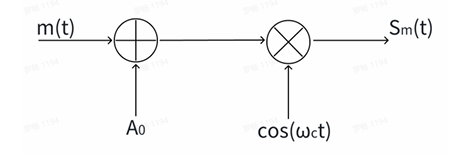
\includegraphics[width=0.6\textwidth]{1.png}
    \caption{AM调制模型}
    \label{img:1}
\end{figure}
AM调制模型原理图如图\ref{img:1}所示
根据AM调制模型,在Multisim中搭建仿真电路如图\ref{img:2}所示,
\begin{figure}[htbp]
    \centering
    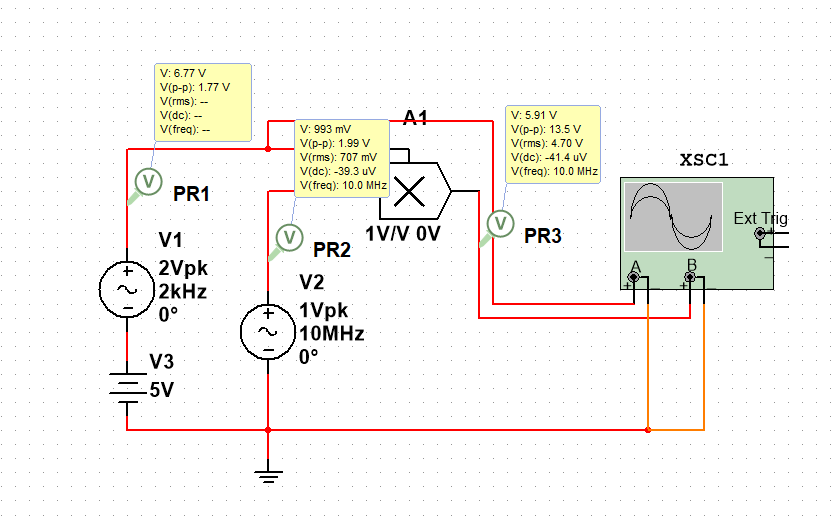
\includegraphics[width=0.6\textwidth]{2.png}
    \caption{AM调制仿真电路图}
    \label{img:2}
\end{figure}
其中$V_1$是单频调制信号,$V_2$是载波信号,$V_3$是直流偏置
\subsection{抑制载波双边带调幅}
\begin{figure}[htbp]
    \centering
    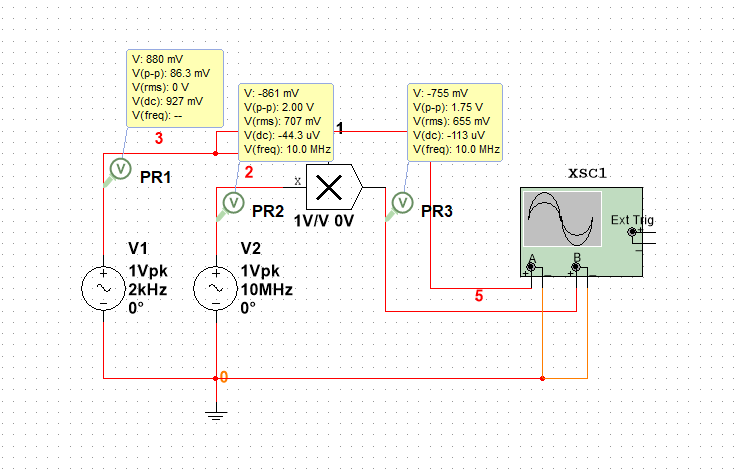
\includegraphics[width=0.6\textwidth]{3.png}
    \caption{DSB调制仿真电路图}
    \label{img:3}
\end{figure}
抑制载波双边带调幅调制模型与AM调制模型相比,仅仅少了直流偏置,如图\ref{img:3}所示为在Multisim中搭建的仿真电路。
\subsection{包络检波}
包络检波电路原理图如图\ref{img:4}所示
\begin{figure}[htbp]
    \centering
    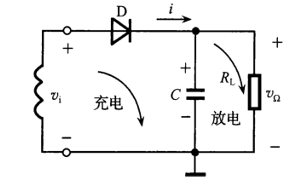
\includegraphics[width=0.6\textwidth]{4.png}
    \caption{包络检波原理电路}
    \label{img:4}
\end{figure}
根据原理电路,在Multisim中绘制包络检波仿真电路图如图\ref{img:5}所示:
\begin{figure}[htbp]
    \centering
    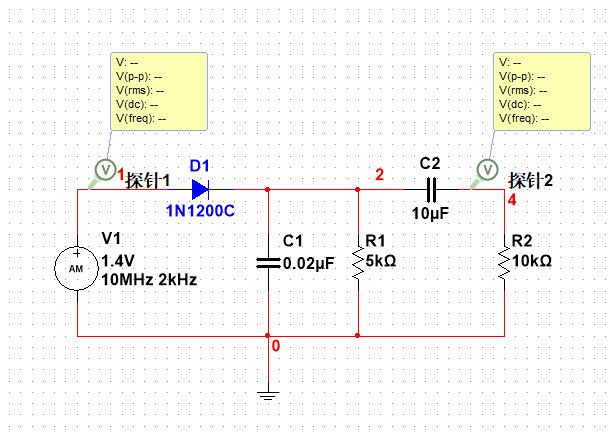
\includegraphics[width=0.6\textwidth]{5.png}
    \caption{包络检波仿真电路图}
    \label{img:5}
\end{figure}
\subsection{同步检波}
同步检波的模型原理图如图\ref{img:6}所示
\begin{figure}[htbp]
    \centering
    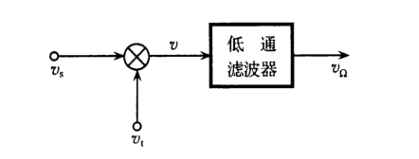
\includegraphics[width=0.6\textwidth]{6.png}
    \caption{同步检波模型图}
    \label{img:6}
\end{figure}
其中$v_s$是输入调幅信号,$v_t$是同步参考信号,根据同步检波模型,在Multisim中绘制同步检波仿真电路图如图\ref{img:7}所示:
\begin{figure}[htbp]
    \centering
    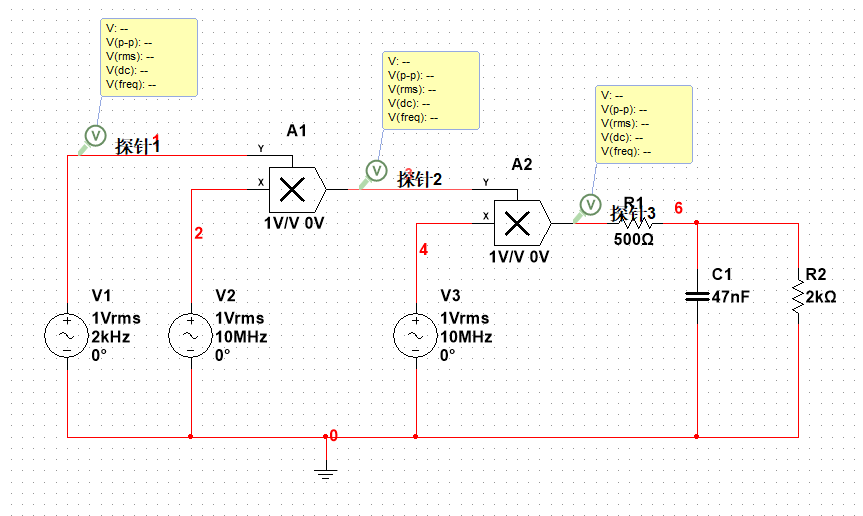
\includegraphics[width=0.6\textwidth]{7.png}
    \caption{同步检波仿真电路图}
    \label{img:7}
\end{figure}
\section{实验步骤}
\begin{itemize}
    \item 按照实验原理图,分别搭建仿真实验电路;
    \item 观察时域波形:使用瞬态分析,添加关键节点的电压信号作为观察量,启动仿真;
    \item 观察频域特性:使用傅里叶分析,分别对关键节点的信号使用傅里叶分析,观察其频谱;
    \item 对于AM调制仿真,更改$V_3$的值,重启瞬态分析,观察时域波形的变化。
\end{itemize}
\section{实验结果与分析}
\subsection{AM}
\subsubsection{时域波形与频谱}
对上述搭建的AM调制仿真电路启动瞬态分析,得到载波信号$V_3$(PR2)、单频调制信号$V_1$(PR1)
和输出信号$V_4$(PR3)的波形如图\ref{img:8}所示
\begin{figure}[htbp]
    \centering
    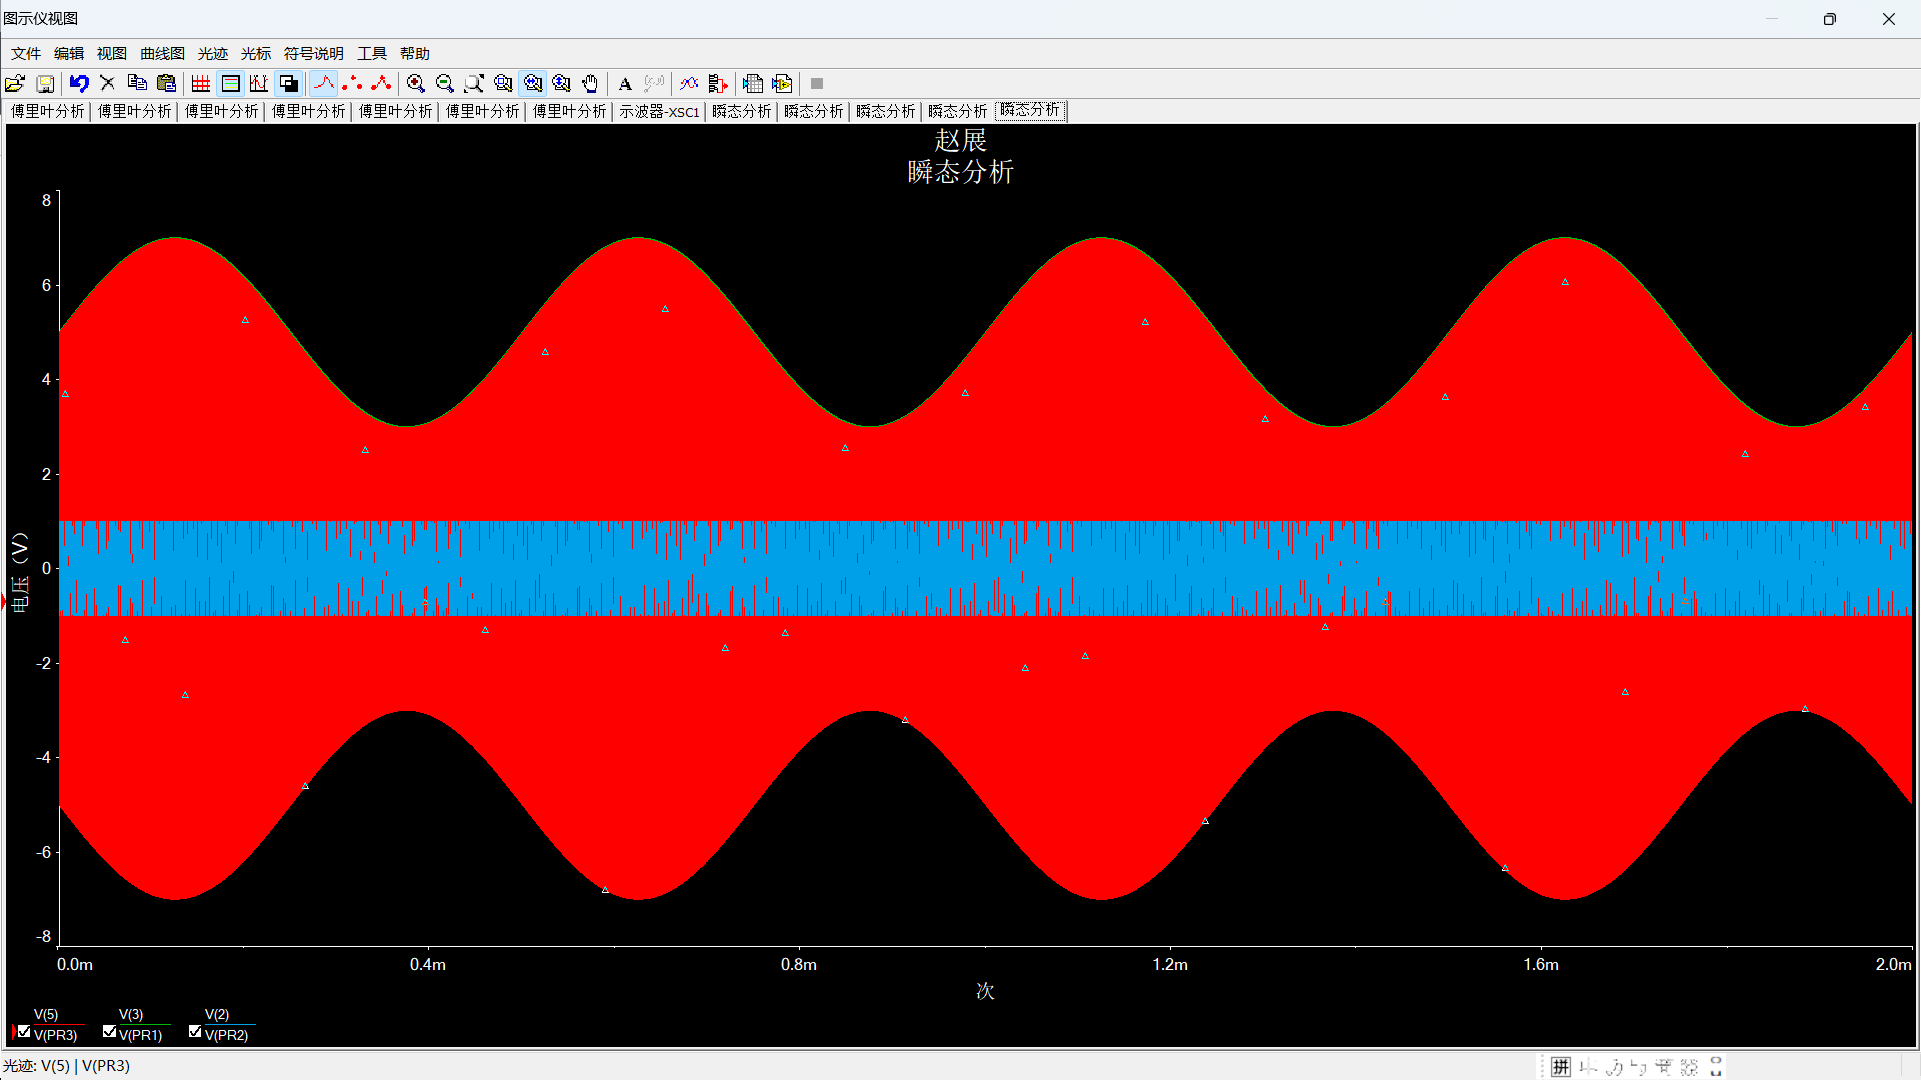
\includegraphics[width=0.6\textwidth]{8.png}
    \caption{瞬态分析:AM}
    \label{img:8}
\end{figure}
启动傅里叶分析,得到的单频调制信号、载波信号和输出信号的频谱如图\ref{img:9},\ref{img:10},\ref{img:11}所示
\begin{figure}[htbp]
    \centering
    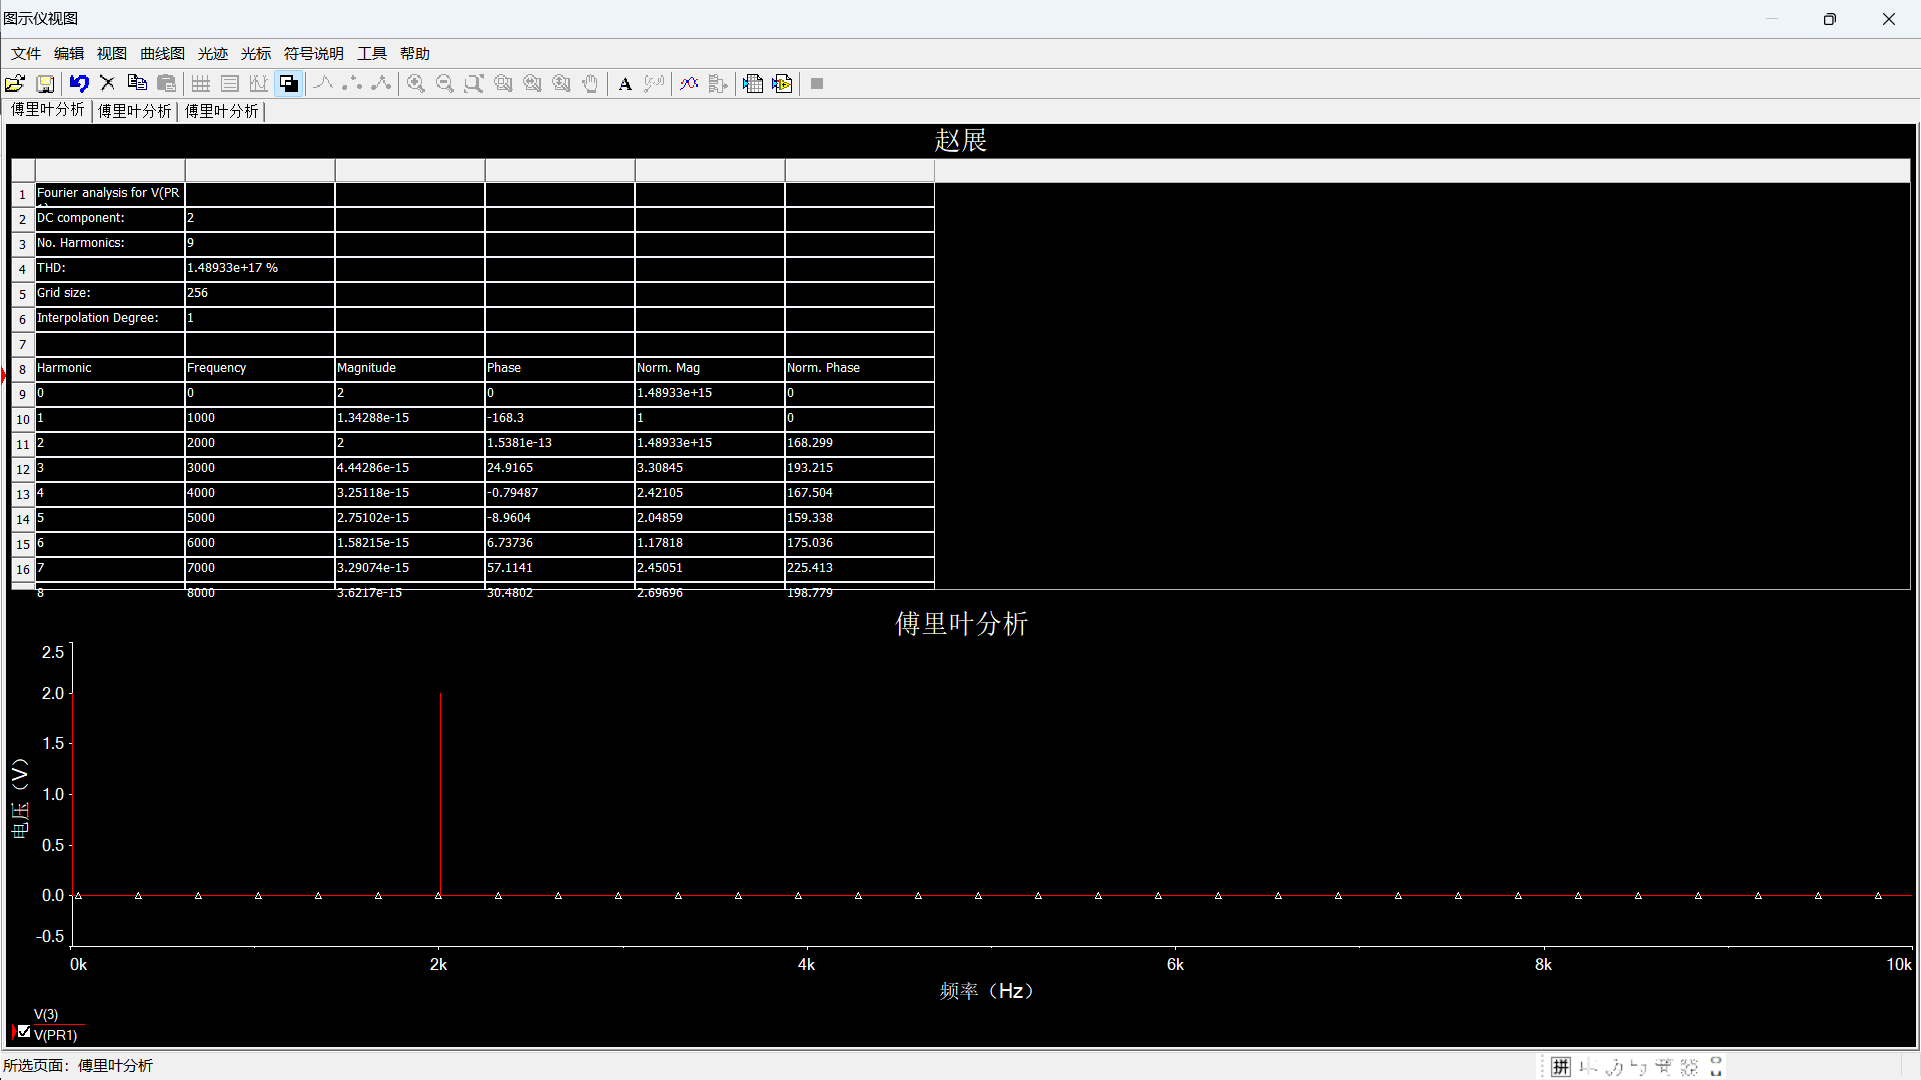
\includegraphics[width=0.6\textwidth]{9.png}
    \caption{傅里叶分析:单频调制信号}
    \label{img:9}
\end{figure}
\begin{figure}[htbp]
    \centering
    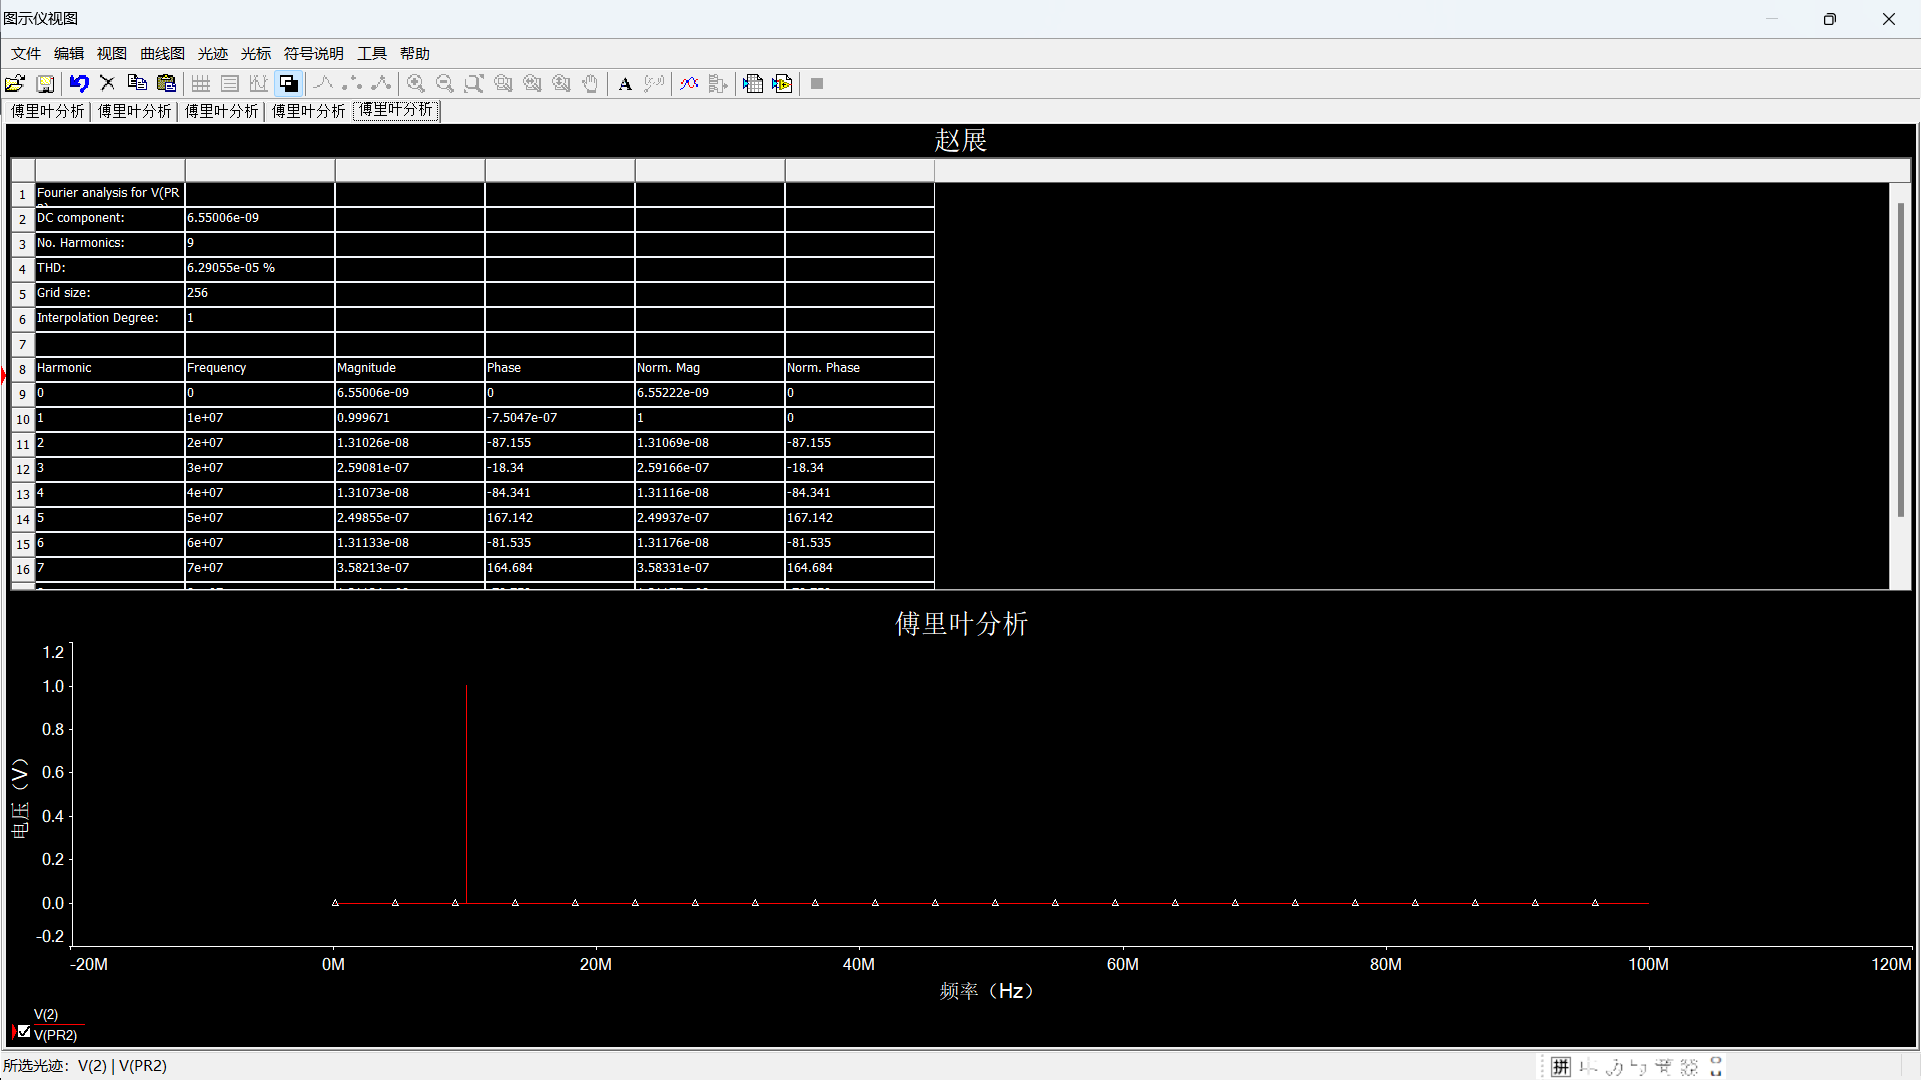
\includegraphics[width=0.6\textwidth]{10.png}
    \caption{傅里叶分析:载波信号}
    \label{img:10}
\end{figure}
\begin{figure}[htbp]
    \centering
    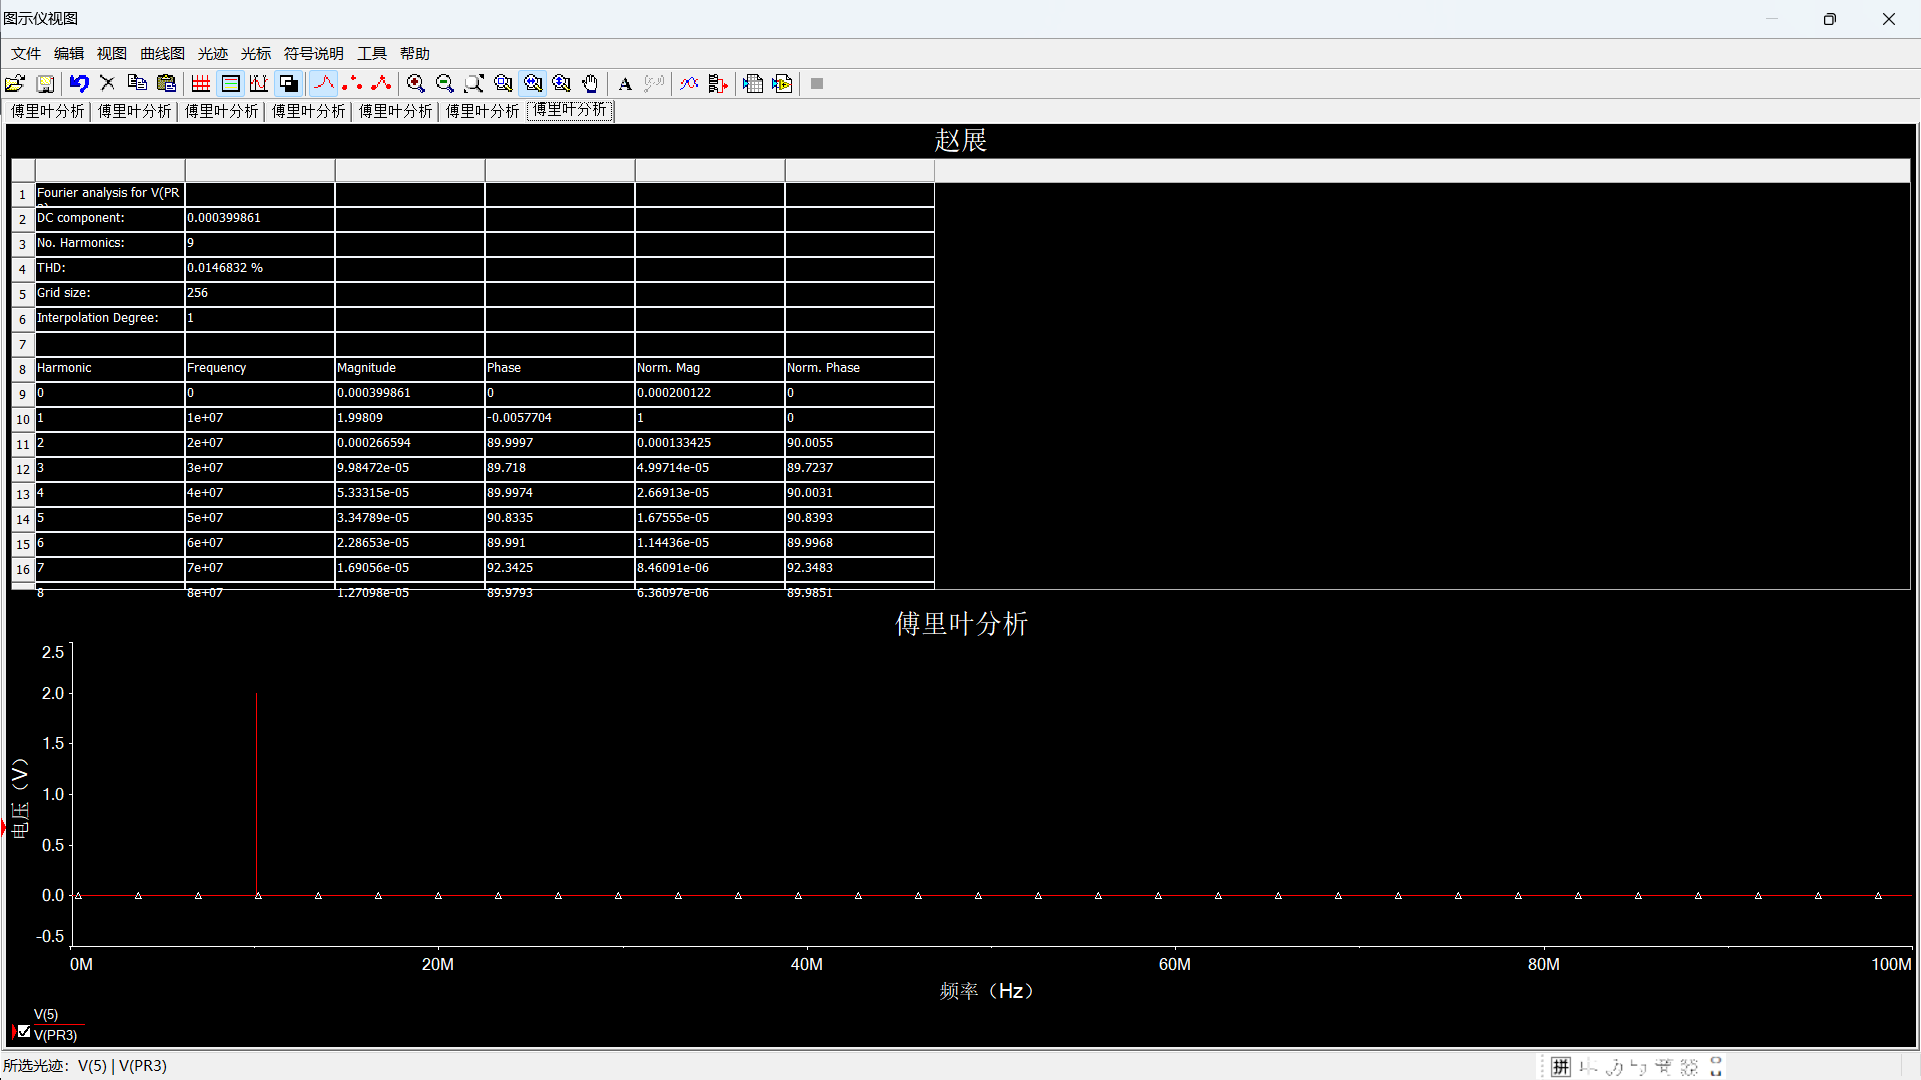
\includegraphics[width=0.6\textwidth]{11.png}
    \caption{傅里叶分析:输出信号}
    \label{img:11}
\end{figure}
可以看到,单频调制信号的频谱为2KHz,载波信号的频谱为10MHz,输出信号的频谱也为10MHz,均表现正确。
\subsubsection{调幅指数对输出的影响}
减少直流偏置的电压值为1V,再次进行瞬态分析,得到如图\ref{img:12}所示的结果。
可以看出此时出现了过调幅状态,此时就不能用包络检波。但是可以使用相干解调。
\subsection{抑制载波双边带调幅}
根据上述搭建的DSB调制仿真电路,进行瞬态分析,得到载波信号、单频调制信号
和输出信号的波形如图\ref{img:13}所示。
\begin{figure}[htbp]
    \centering
    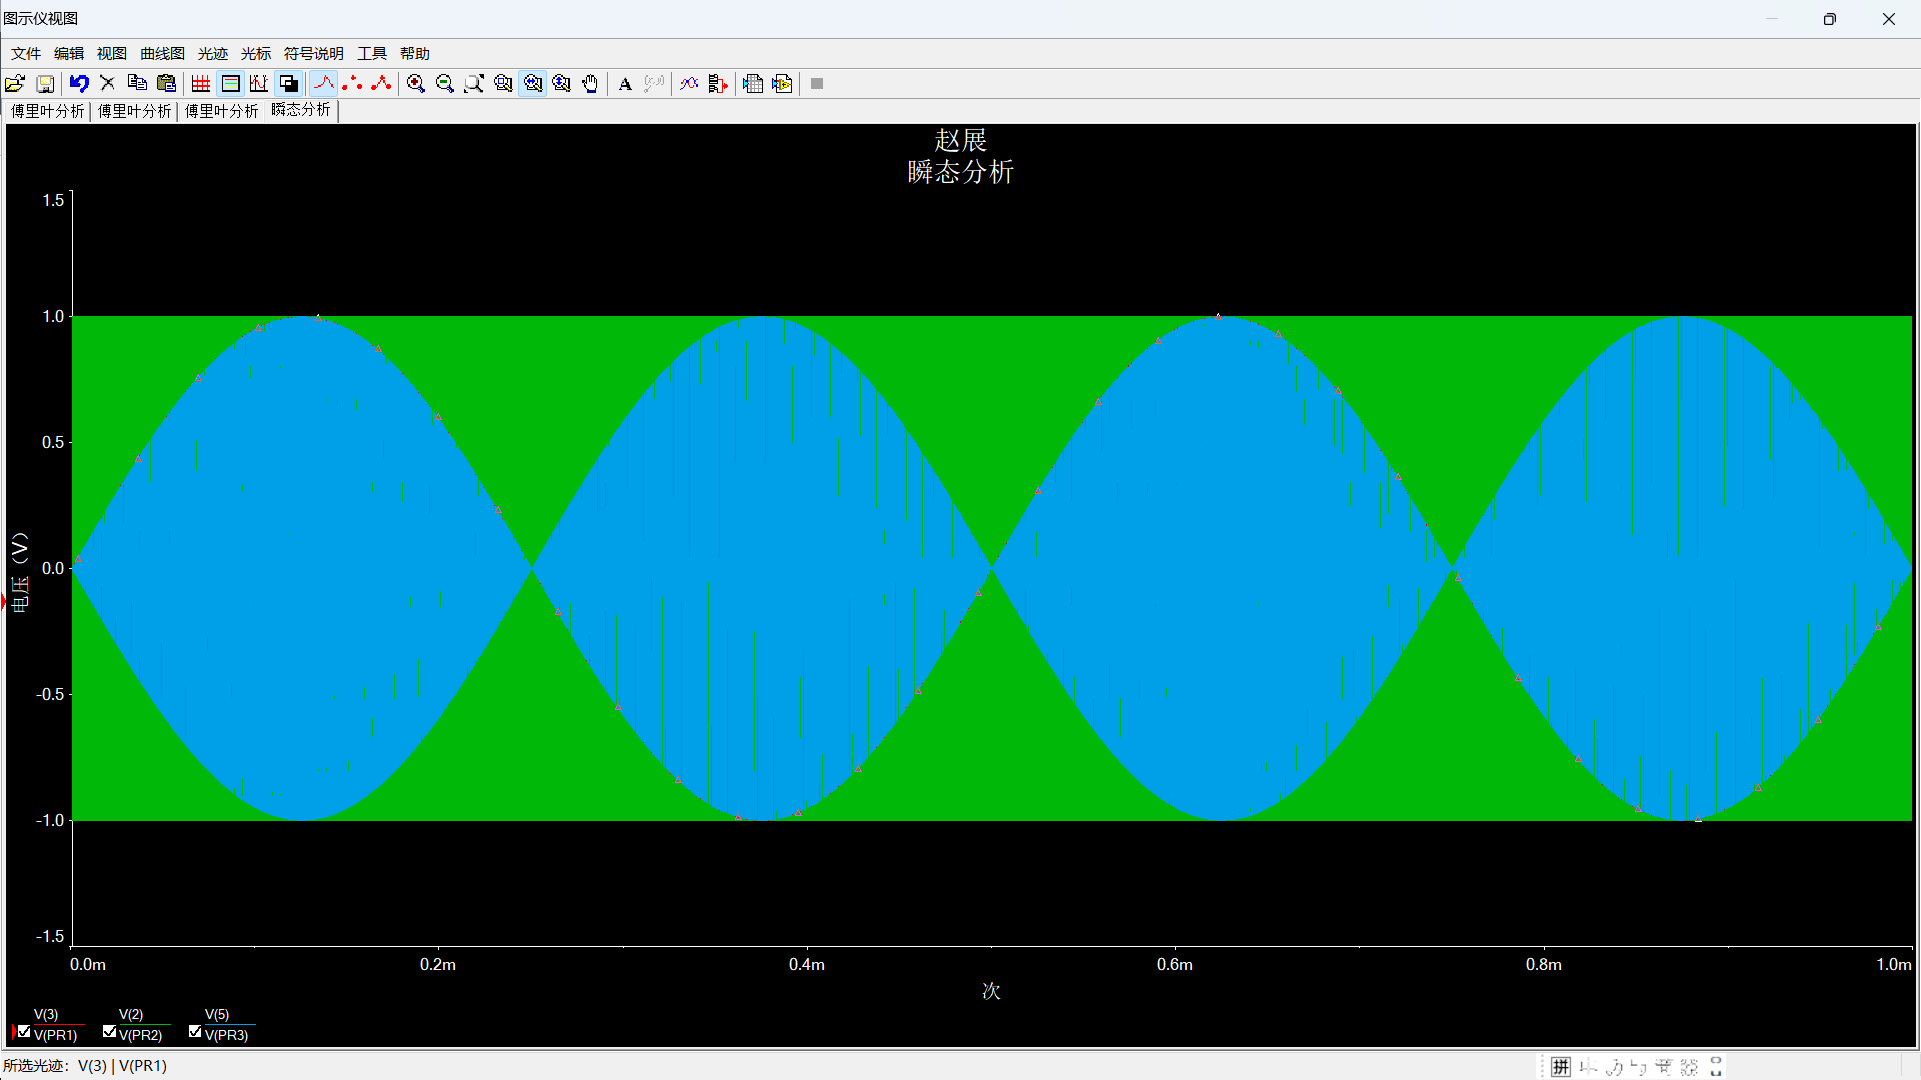
\includegraphics[width=0.6\textwidth]{13.png}
    \caption{瞬态分析:DSB}
    \label{img:13}
\end{figure}
\begin{figure}[htbp]
    \centering
    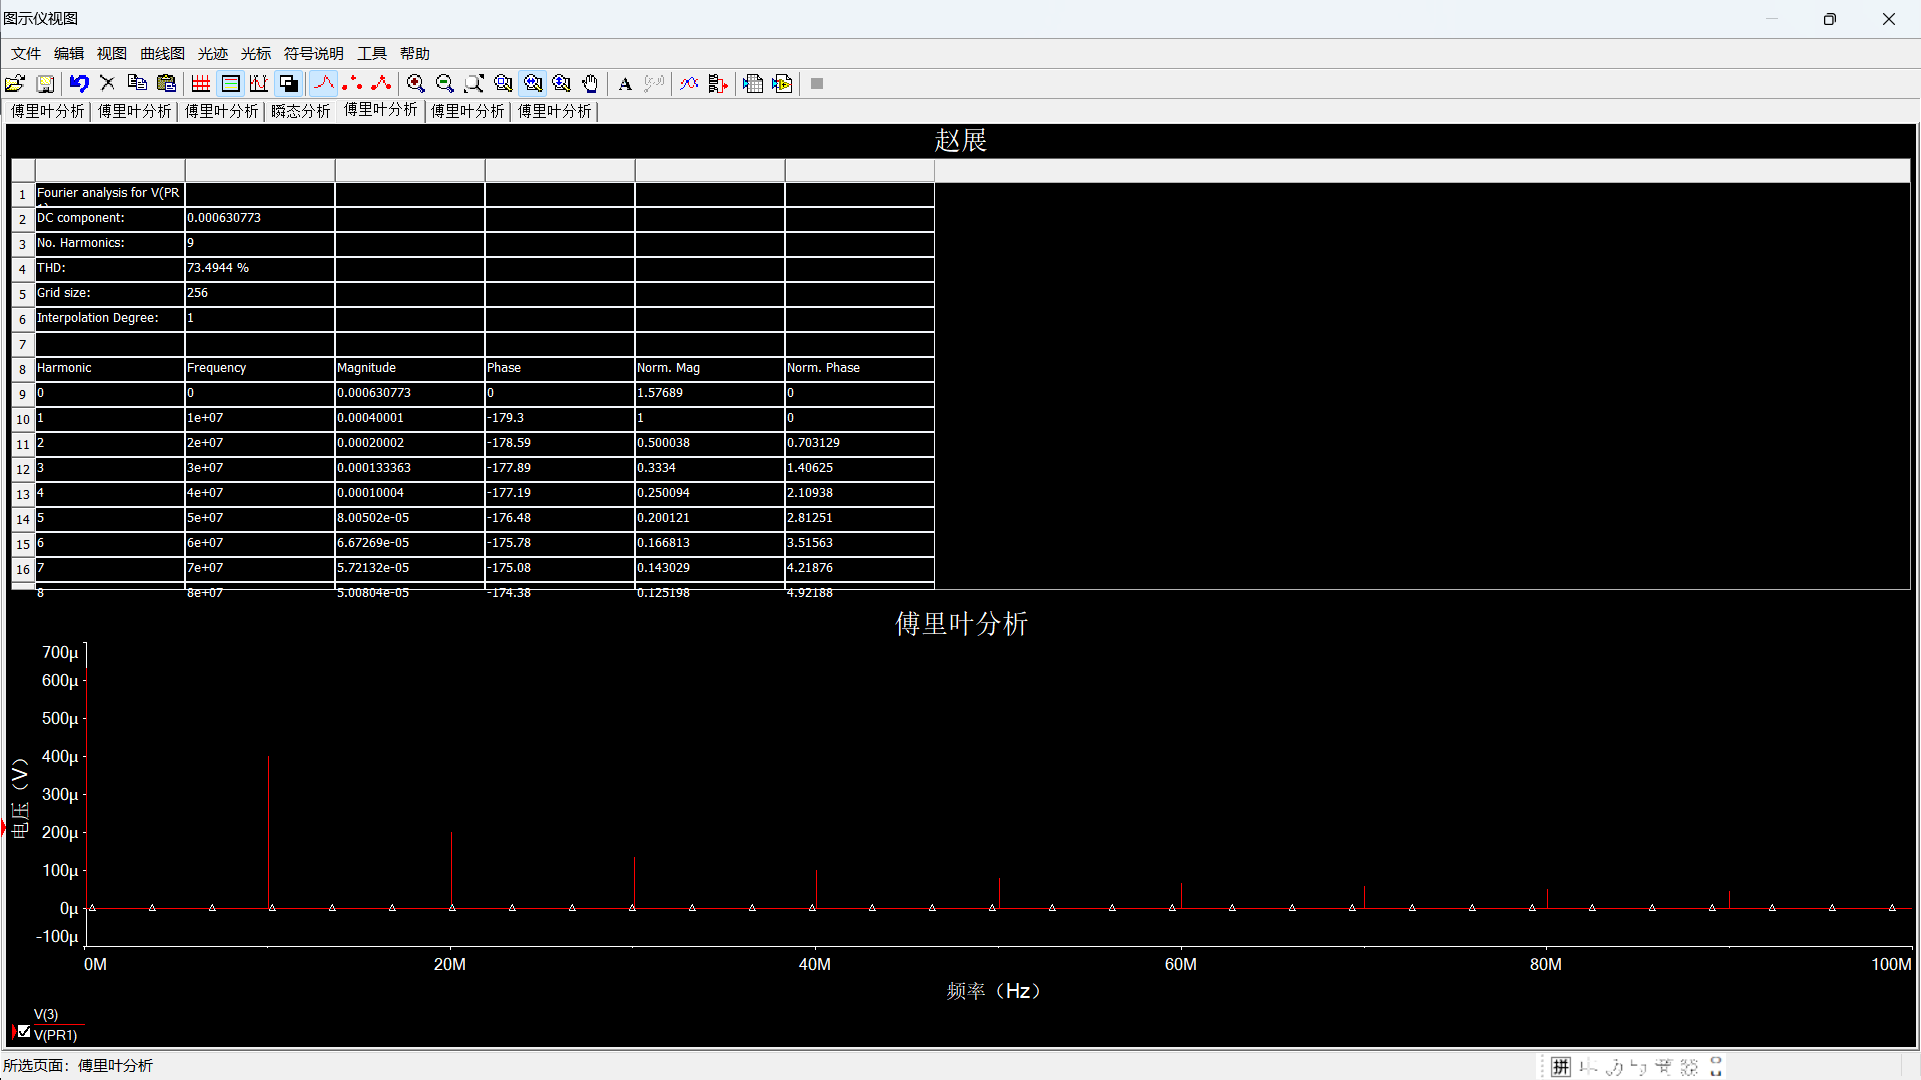
\includegraphics[width=0.6\textwidth]{14.png}
    \caption{傅里叶分析:单频调制信号}
    \label{img:14}
\end{figure}
\begin{figure}[htbp]
    \centering
    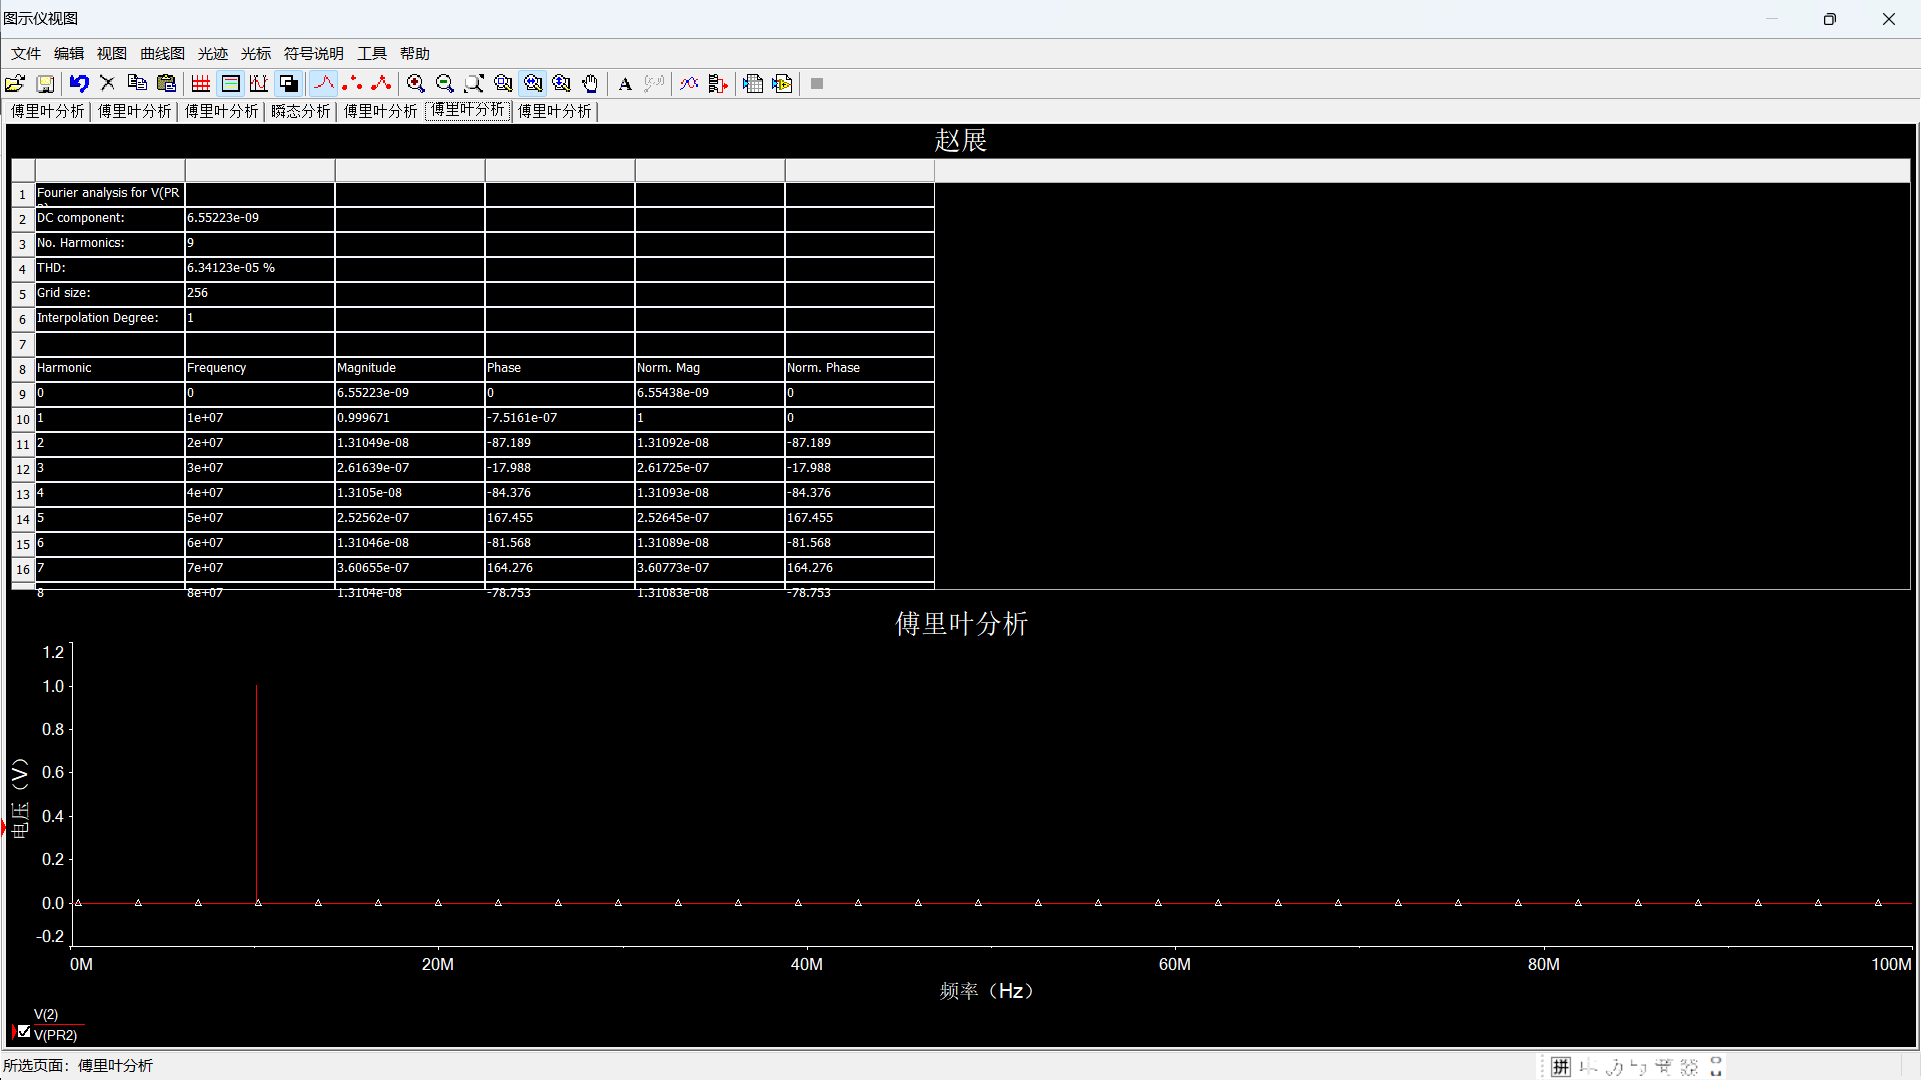
\includegraphics[width=0.6\textwidth]{15.png}
    \caption{傅里叶分析:载波信号}
    \label{img:15}
\end{figure}
\begin{figure}[htbp]
    \centering
    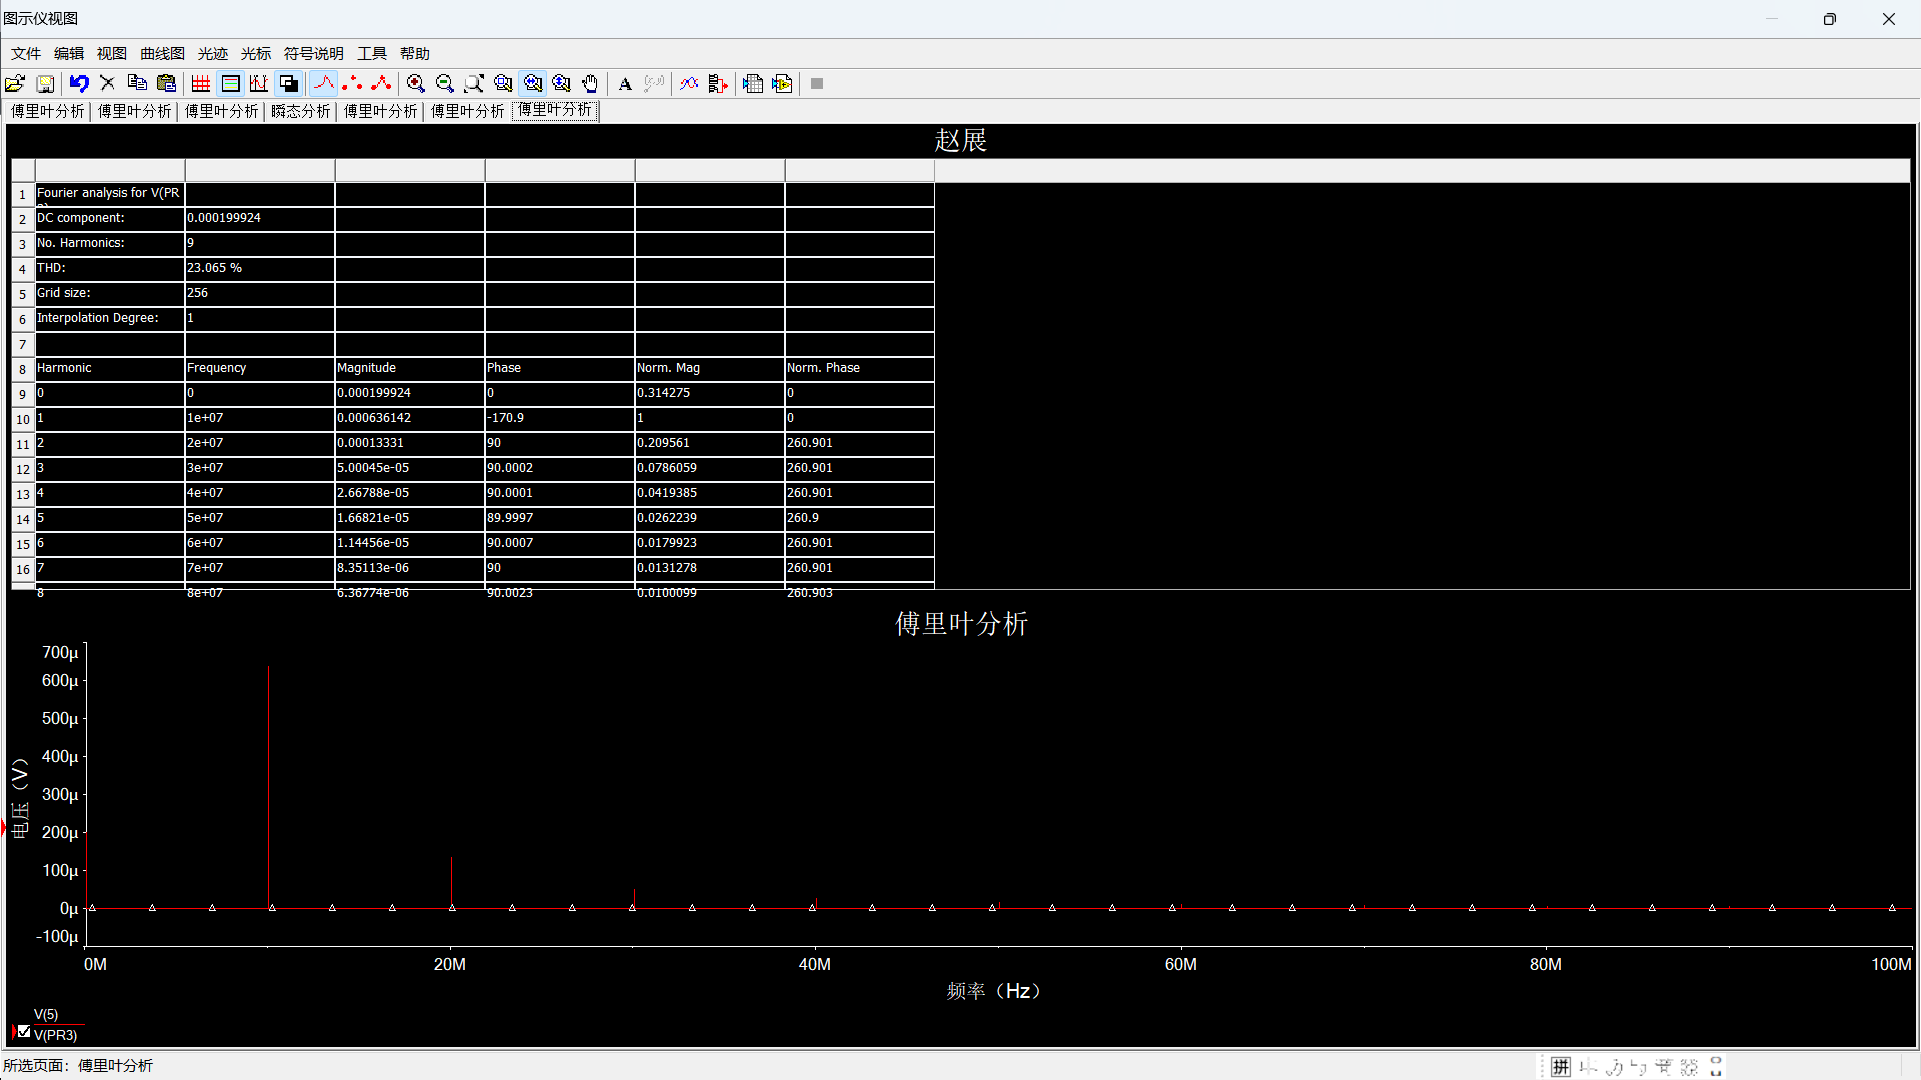
\includegraphics[width=0.6\textwidth]{16.png}
    \caption{傅里叶分析:输出信号}
    \label{img:16}
\end{figure}
进行傅里叶分析,同样添加载波信号、单频调制信号和输出信号为观察量,得到频
谱图如图\ref{img:14},\ref{img:15},\ref{img:16}所示。
和AM同样均表现正确。

\subsection{包络检波}
根据上述搭建的包络检波仿真电路,进行瞬态分析,得到输入已调信号和输出解调信号的波形如图\ref{img:17}所示:
\begin{figure}[htbp]
    \centering
    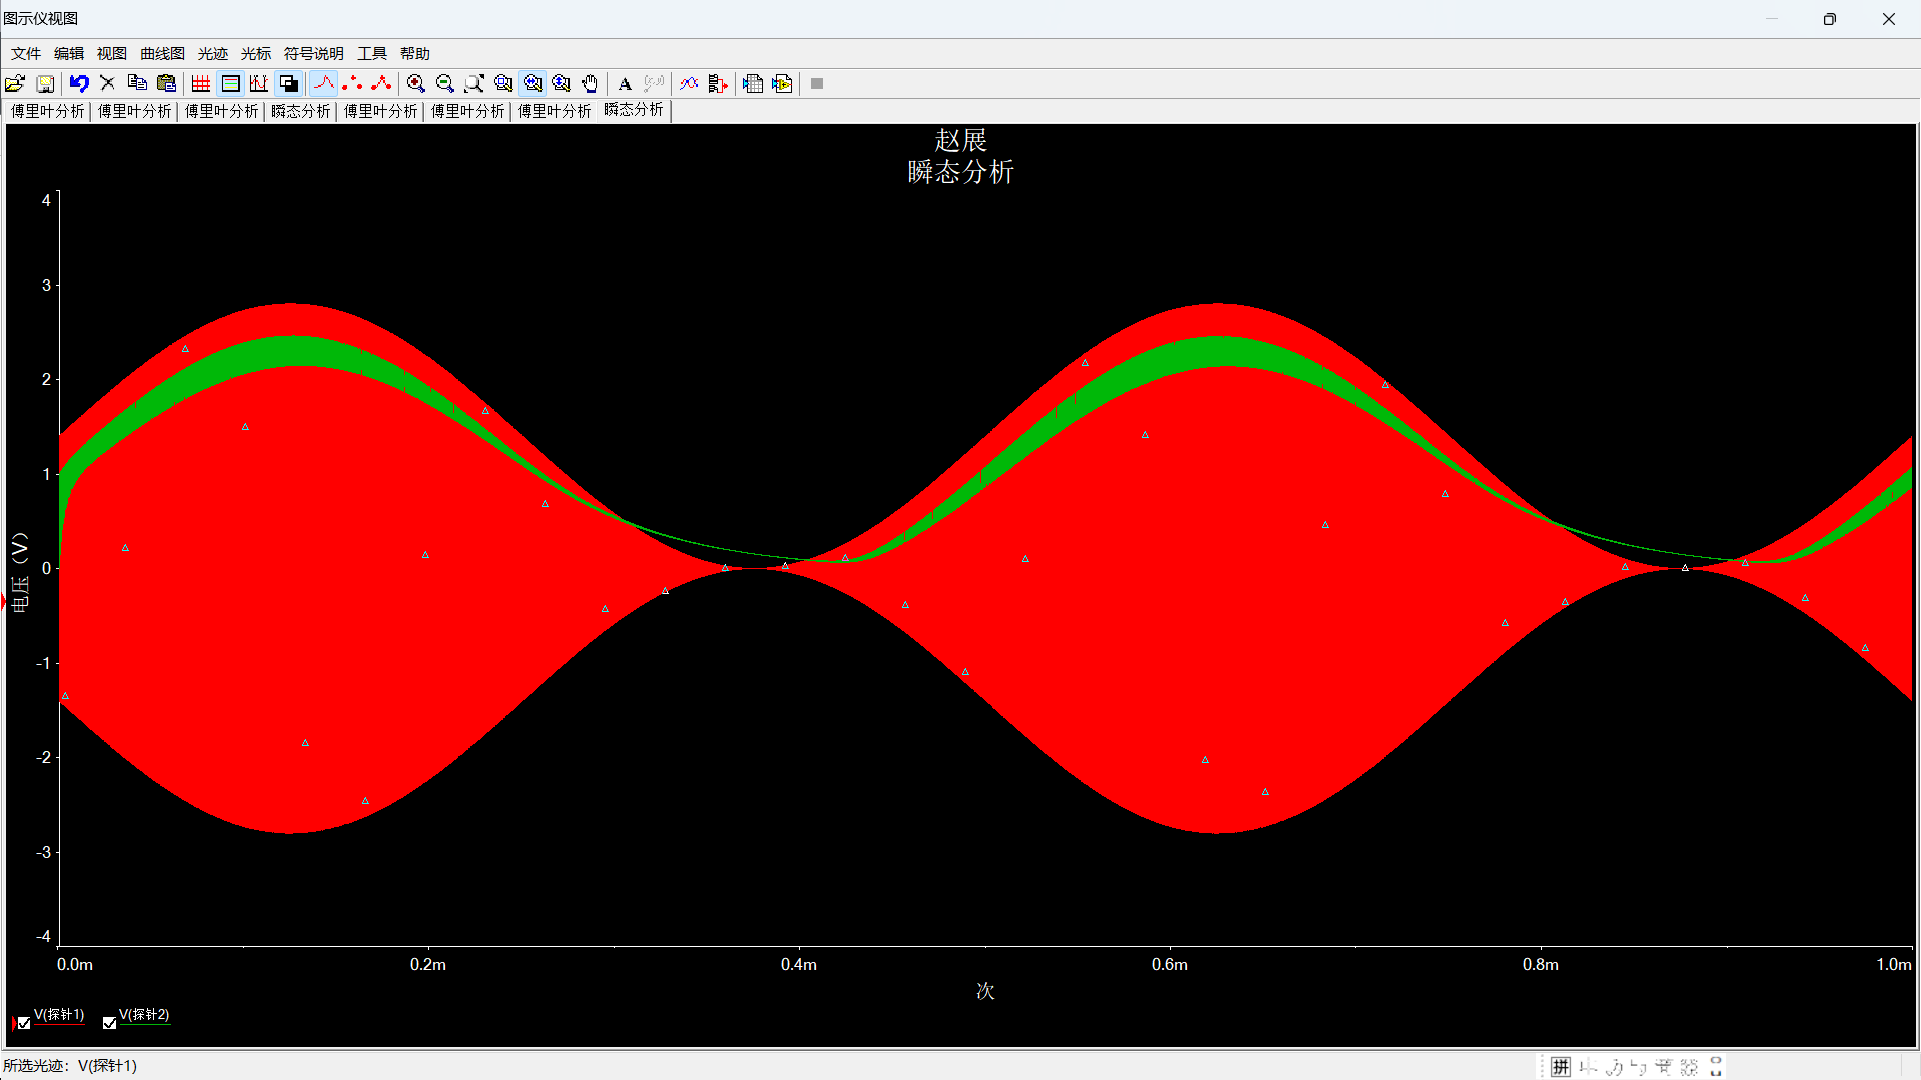
\includegraphics[width=0.6\textwidth]{17.png}
    \caption{瞬态分析:包络检波}
    \label{img:17}
\end{figure}
同时也可以进行傅里叶分析得到输入已调信号和输出调制信号如图\ref{img:18},\ref{img:19}所示。
可以看到,输出调制信号的频谱集中在2KHz附近,输入已调信号大部分集中在10MHz附
近,频谱表现正确
\subsection{同步检波}
根据上述搭建的同步检波仿真电路,进行瞬态分析,得到输入已调信号、输出调制信号
和同步载波信号的波形如图\ref{img:20}所示。
\begin{figure}[htbp]
    \centering
    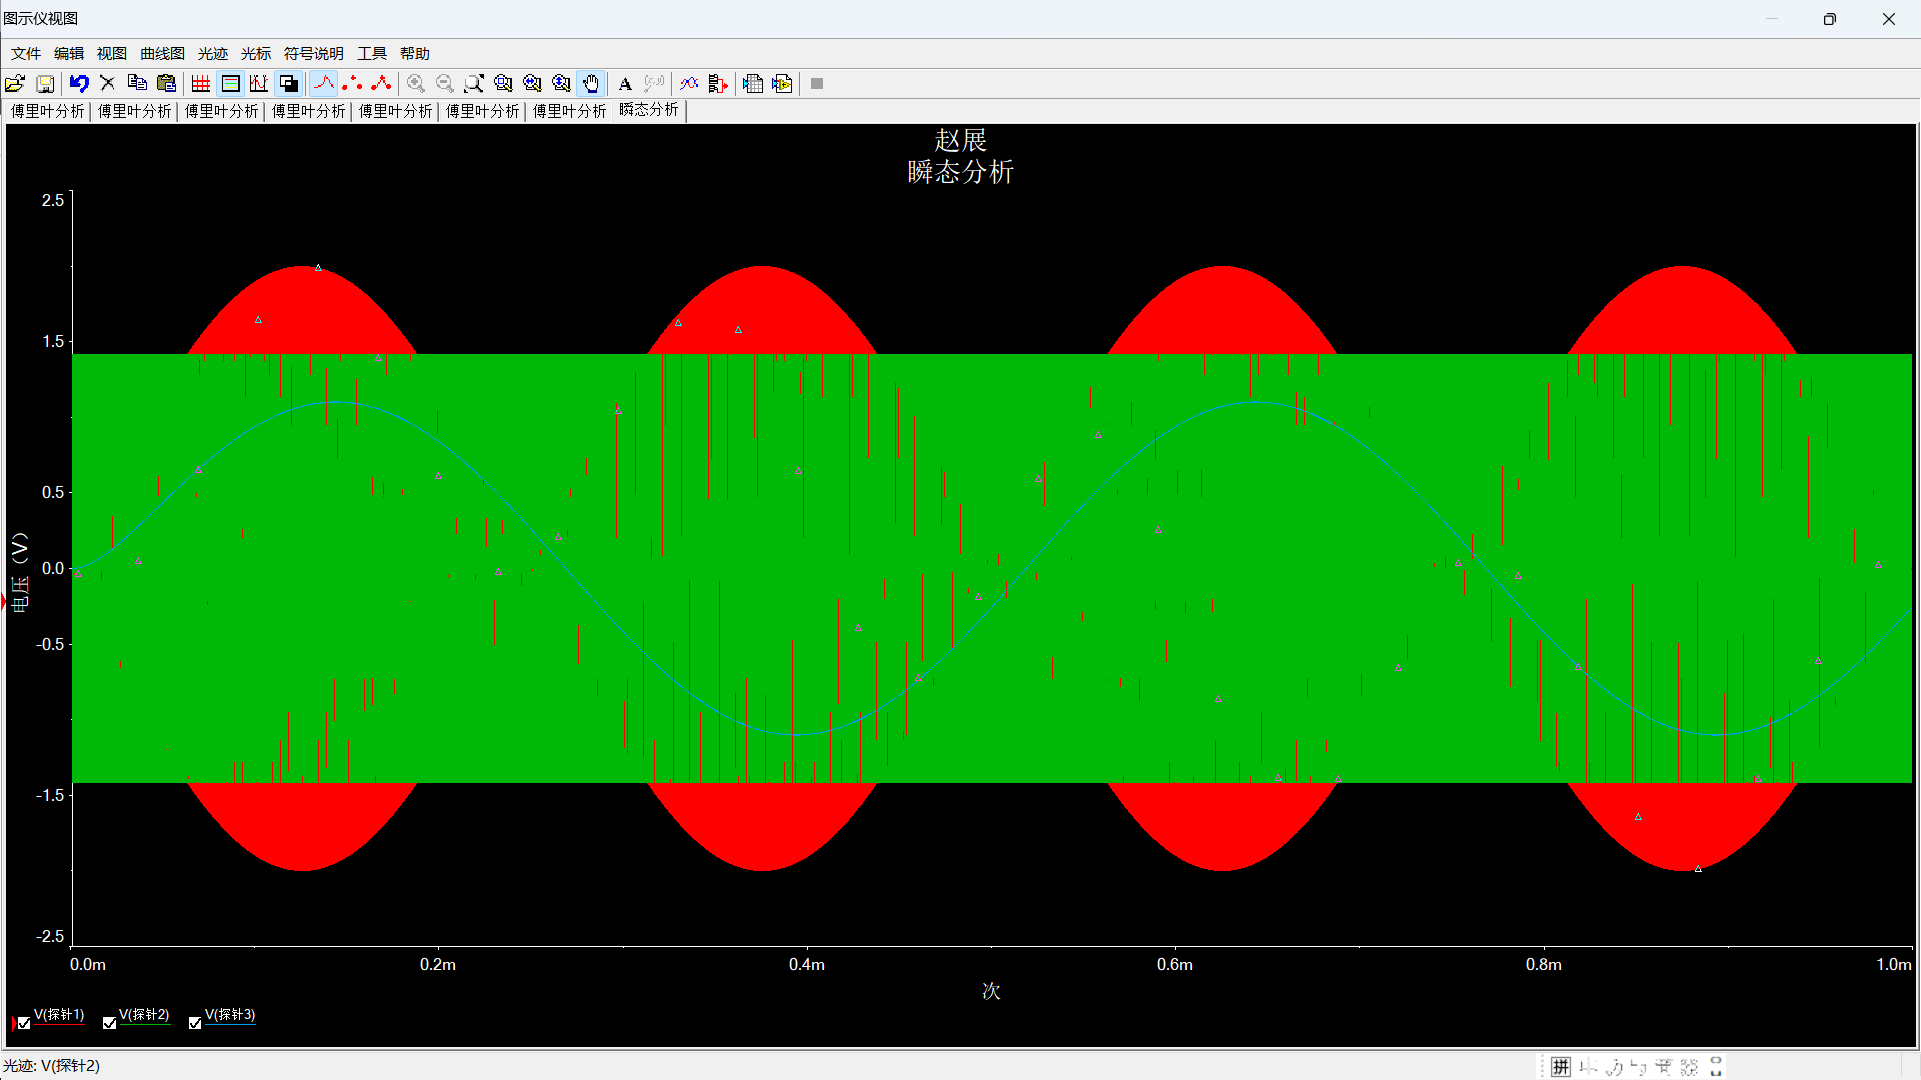
\includegraphics[width=0.6\textwidth]{20.png}
    \caption{瞬态分析:同步检波}
    \label{img:20}
\end{figure}
然后再次进行傅里叶仿真,添加输入已调信号、输出调制信号和同步载波信号为观察量,得
到频谱图如图\ref{img:21},\ref{img:22},\ref{img:23}所示:
\begin{figure}[htbp]
    \centering
    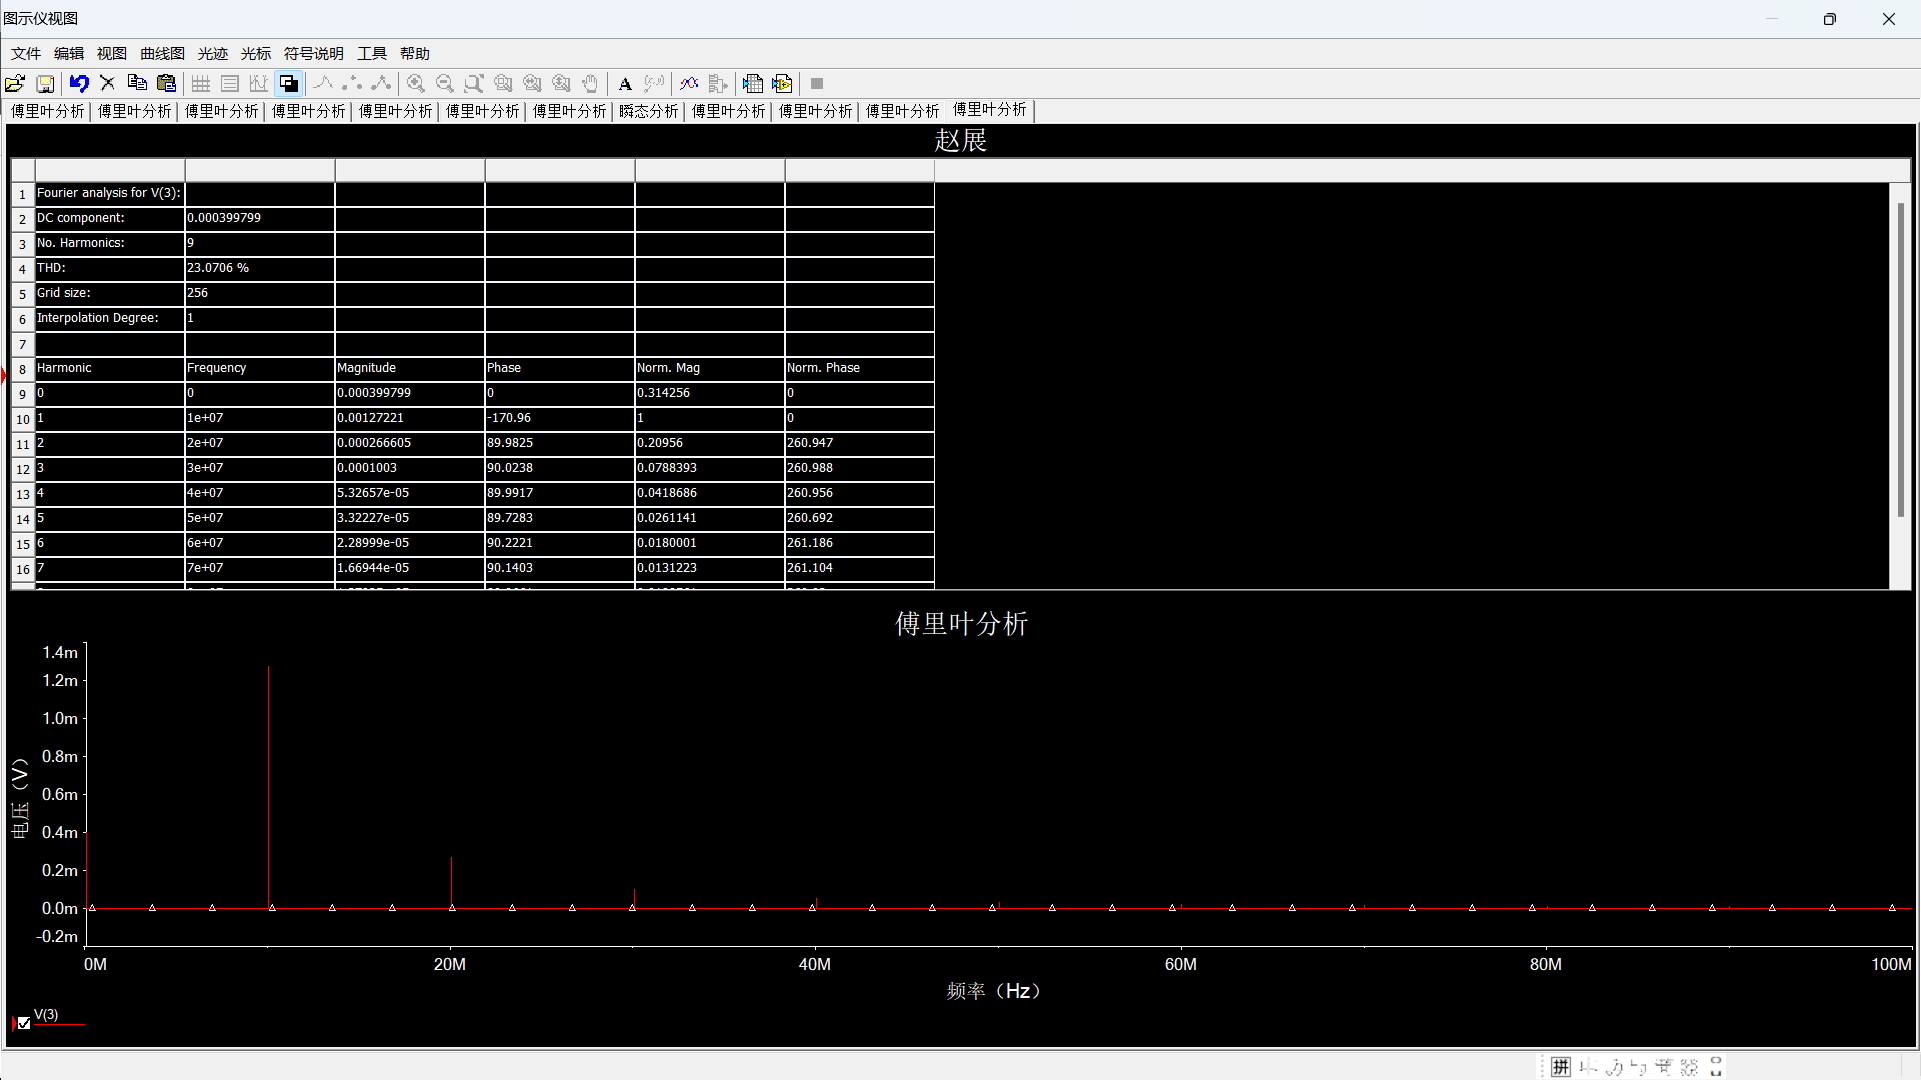
\includegraphics[width=0.6\textwidth]{21.png}
    \caption{傅里叶分析:输入已调信号}
    \label{img:21}
\end{figure}
\begin{figure}[htbp]
    \centering
    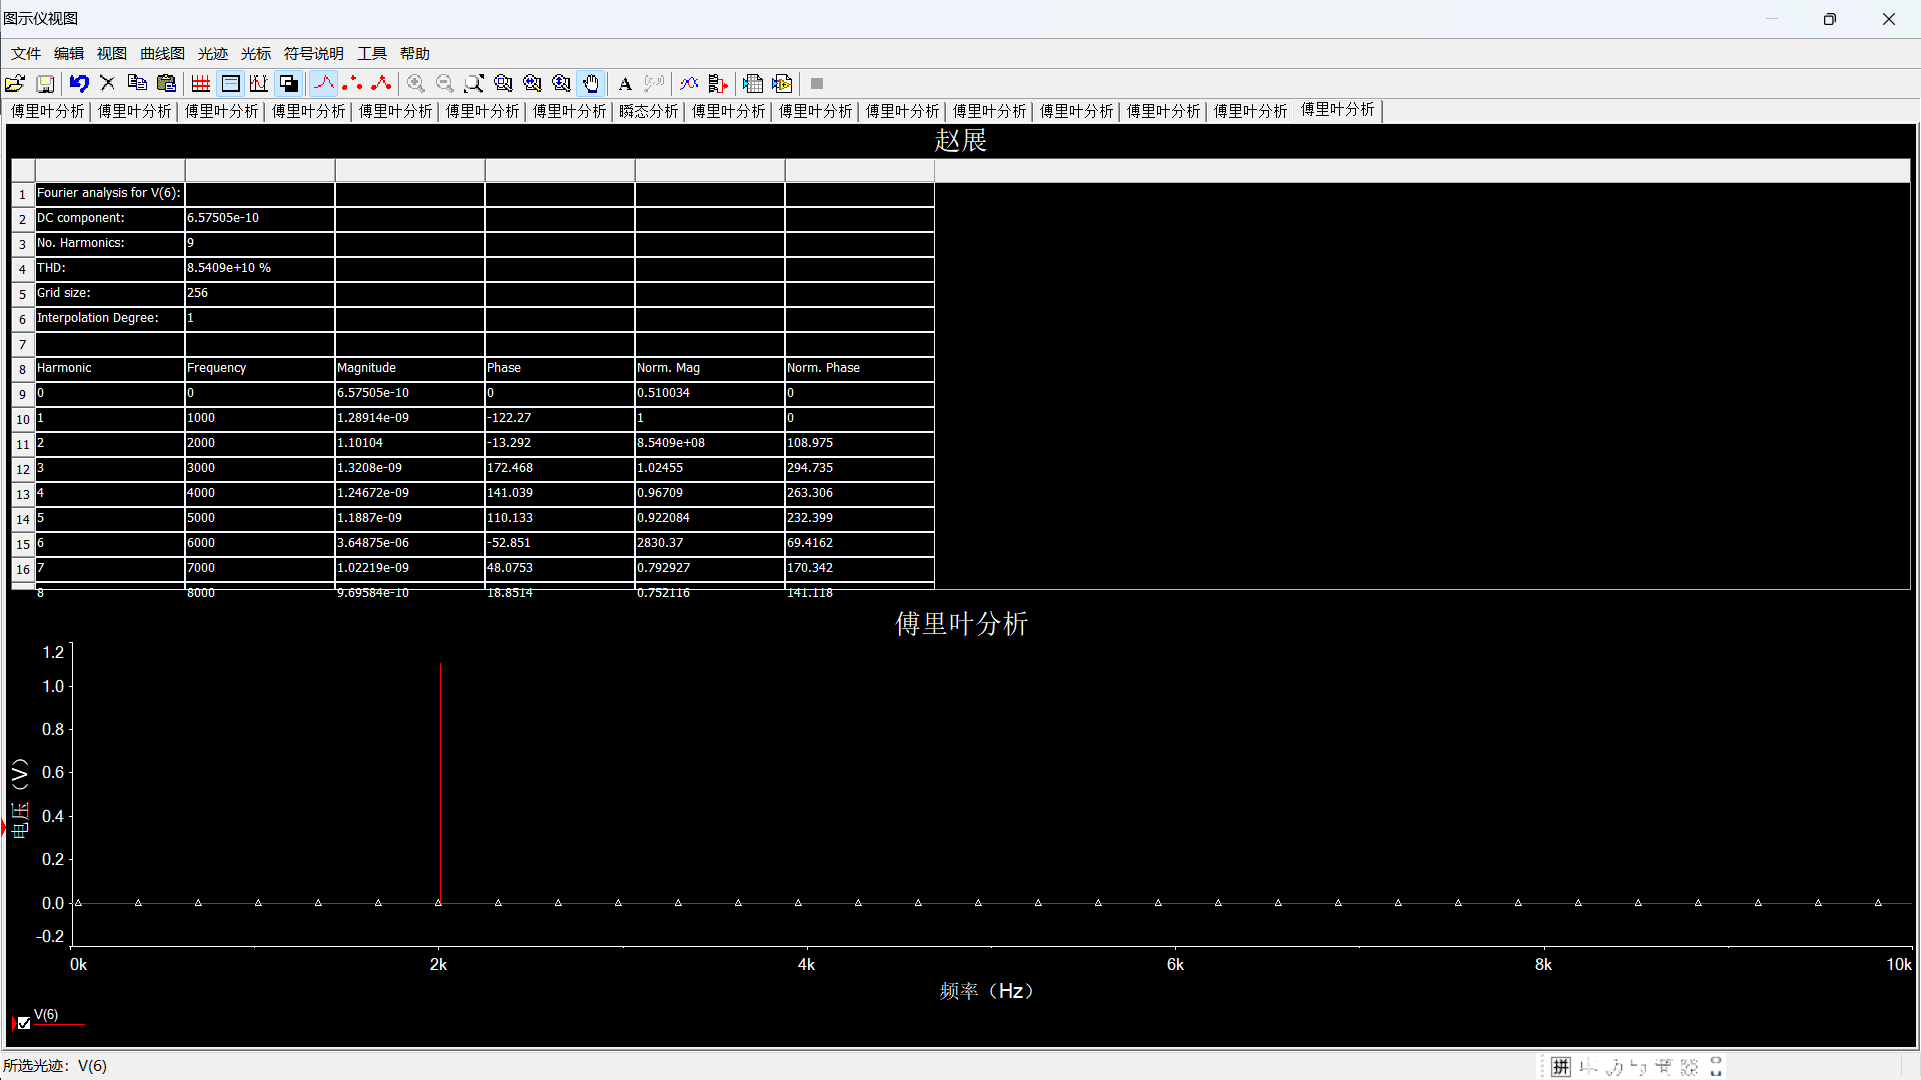
\includegraphics[width=0.6\textwidth]{22.png}
    \caption{傅里叶分析:输出调制信号}
    \label{img:22}
\end{figure}
\begin{figure}[htbp]
    \centering
    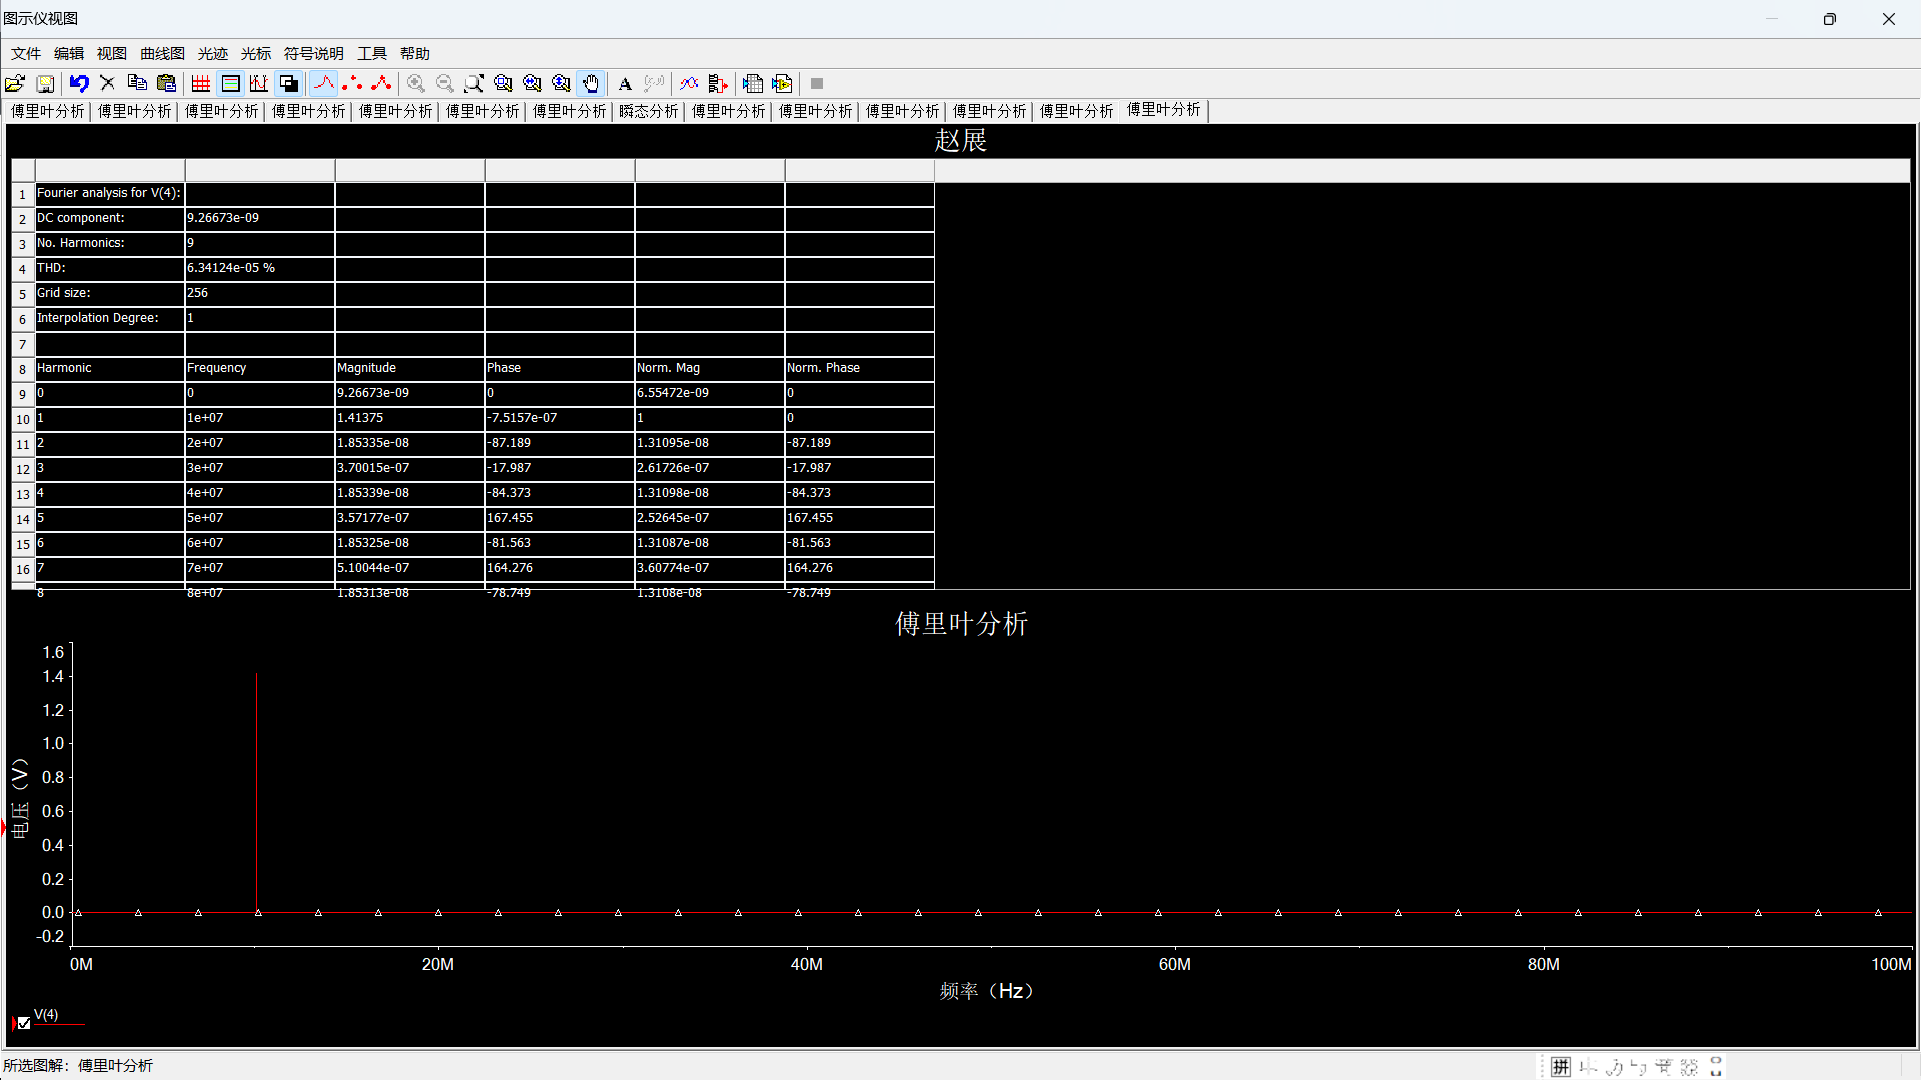
\includegraphics[width=0.6\textwidth]{23.png}
    \caption{傅里叶分析:同步载波信号}
    \label{img:23}
\end{figure}
可以看到,输入已调信号的频谱大部分集中在10MHz附近,输出调制信号的频谱基本就是
2KHz,同步载波信号的频谱只有10MHz部分,频谱表现基本正确。
\section{实验小结}
本实验是通信电子线路最后一次实验,通过这四次的实验,我对multisim仿真工具的使用已经基本熟练,同时也在每次实验之后对相应的知识点进一步的巩固。
说不如做,我想经过这些实验我对这些知识点的记忆会更加深刻。
\end{document}